\section{$\pi^0$ comparison of g12 to g1c}

A total of 177 points in $\cos \theta$ in 33 beam energies were compared between g12 and g1c. The a sample pf such plots can be found in (see section known xsections). The unnormalized pull distribution of the 177 points can be seen in \ref{fig:pi0pull}.
\begin{figure}[htpb]\begin{center}
\includegraphics[width=0.8\columnwidth]{figures/lepton/Pull_trial.eps}
\caption[Unnormalized Pull Distribution Comparison for g1c and g12 $\pi^0$ cross-section]{\label{fig:pi0pull}Unnormalized Pull Distribution Comparison for g1c and g12 $\pi^0$ cross-section.}
\end{center}\end{figure}

The maximum deviation can been attributed to the difference mainly in the forward direction, i.e $\cos \theta = 0.75$, see \ref{fig:pi0pulldev} . This deviation is also where the g1c measurements deviate from other measurements performed outside CLAS.
\begin{figure}[htpb]\begin{center}
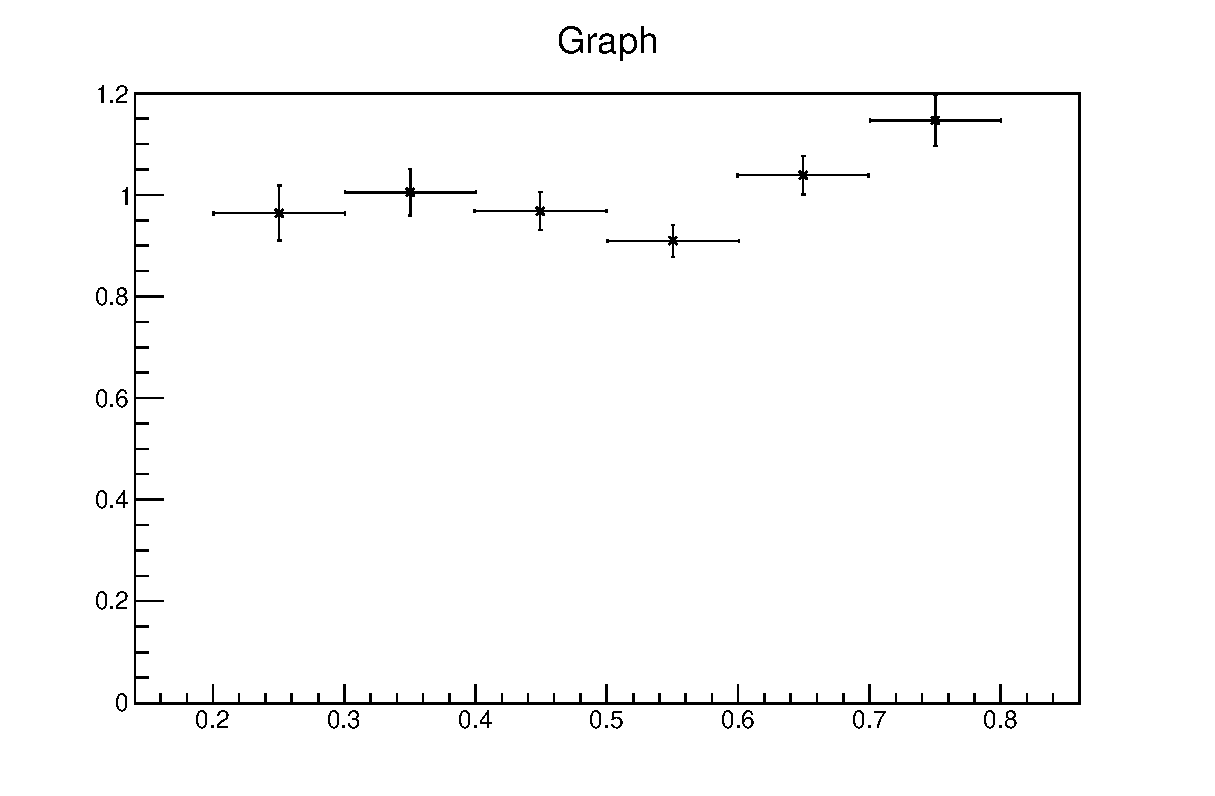
\includegraphics[width=0.8\columnwidth]{figures/lepton/Ratio_inCosTheta.eps}
\caption[Ratio of Standard Deviation for g1c and g12 $\pi^0$ cross-section]{\label{fig:pi0pulldev}Ratio of standard deviation for g1c and g12 $\pi^0$ cross-section.}
\end{center}\end{figure}

